\documentclass[dvipdfmx]{beamer}

\usepackage{beamerthemesplit}
\usepackage[]{graphicx}
\graphicspath{%
{./slide01-img/}%
{./text01-img/}%
}


\usepackage{listings}
\usepackage{hyperref}
\usepackage{pxjahyper}
\usepackage{color}

\setbeamertemplate{footline}[frame number]
\title{子どもIT未来塾 第1回}
\author{塾長 清水尚彦}

\def\quiz{1}

\begin{document}

\frame{
   \begin{center}
    \huge{子どもIT未来塾}\\

    \vspace{48pt}
	   \Large{第1回}\\
	   {\huge\bf ラズベリーパイの使い方・\\
	   \huge\bf 自己紹介ページを作ろう}\\
    \vspace{24pt}
    \large{塾長 清水尚彦}\\
    \vspace{10pt}
    \large{\the\year 年 6月24日}
  \end{center}
}



\begin{frame}[fragile]
	\frametitle{3時間目:ラズベリーパイになれよう(2) P.36-43~~~\raisebox{-3mm}{
\includegraphics[width=0.1\textwidth]{raspberry}}}
    \begin{description}
      \item[ラズベリーパイのいろいろな機能をつかっていこう]
    \end{description}
    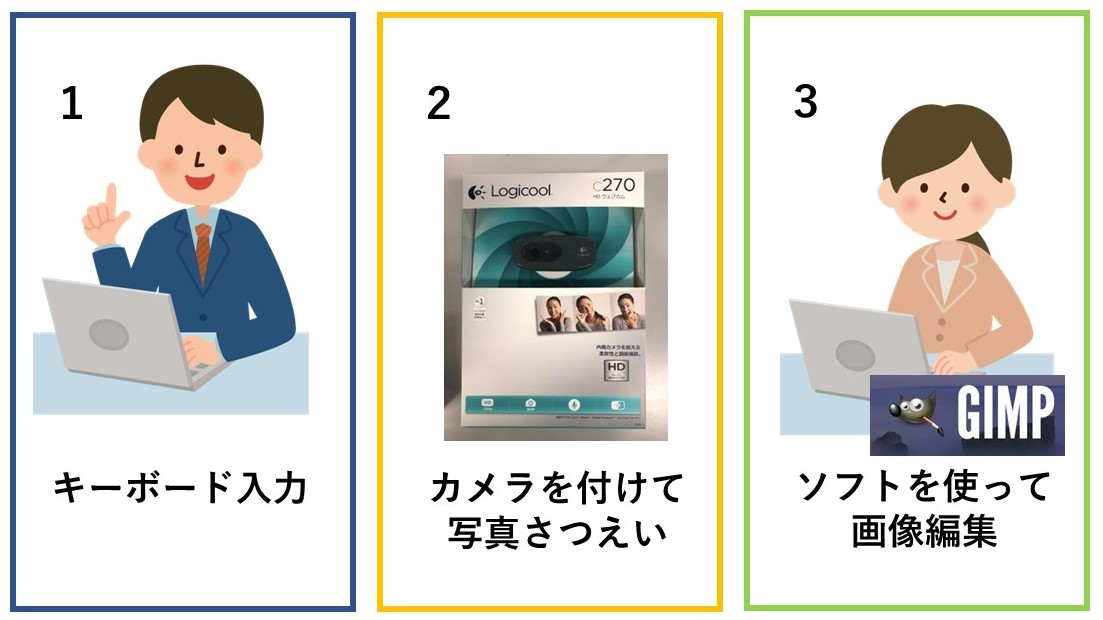
\includegraphics[width=\textwidth]{slide03_002.jpg}
\end{frame}

\begin{frame}[fragile]
	\frametitle{例題1-16 カメラで写真をさつえいしよう P.36-39~~~\raisebox{-3mm}{
\includegraphics[width=0.1\textwidth]{raspberry}}}
    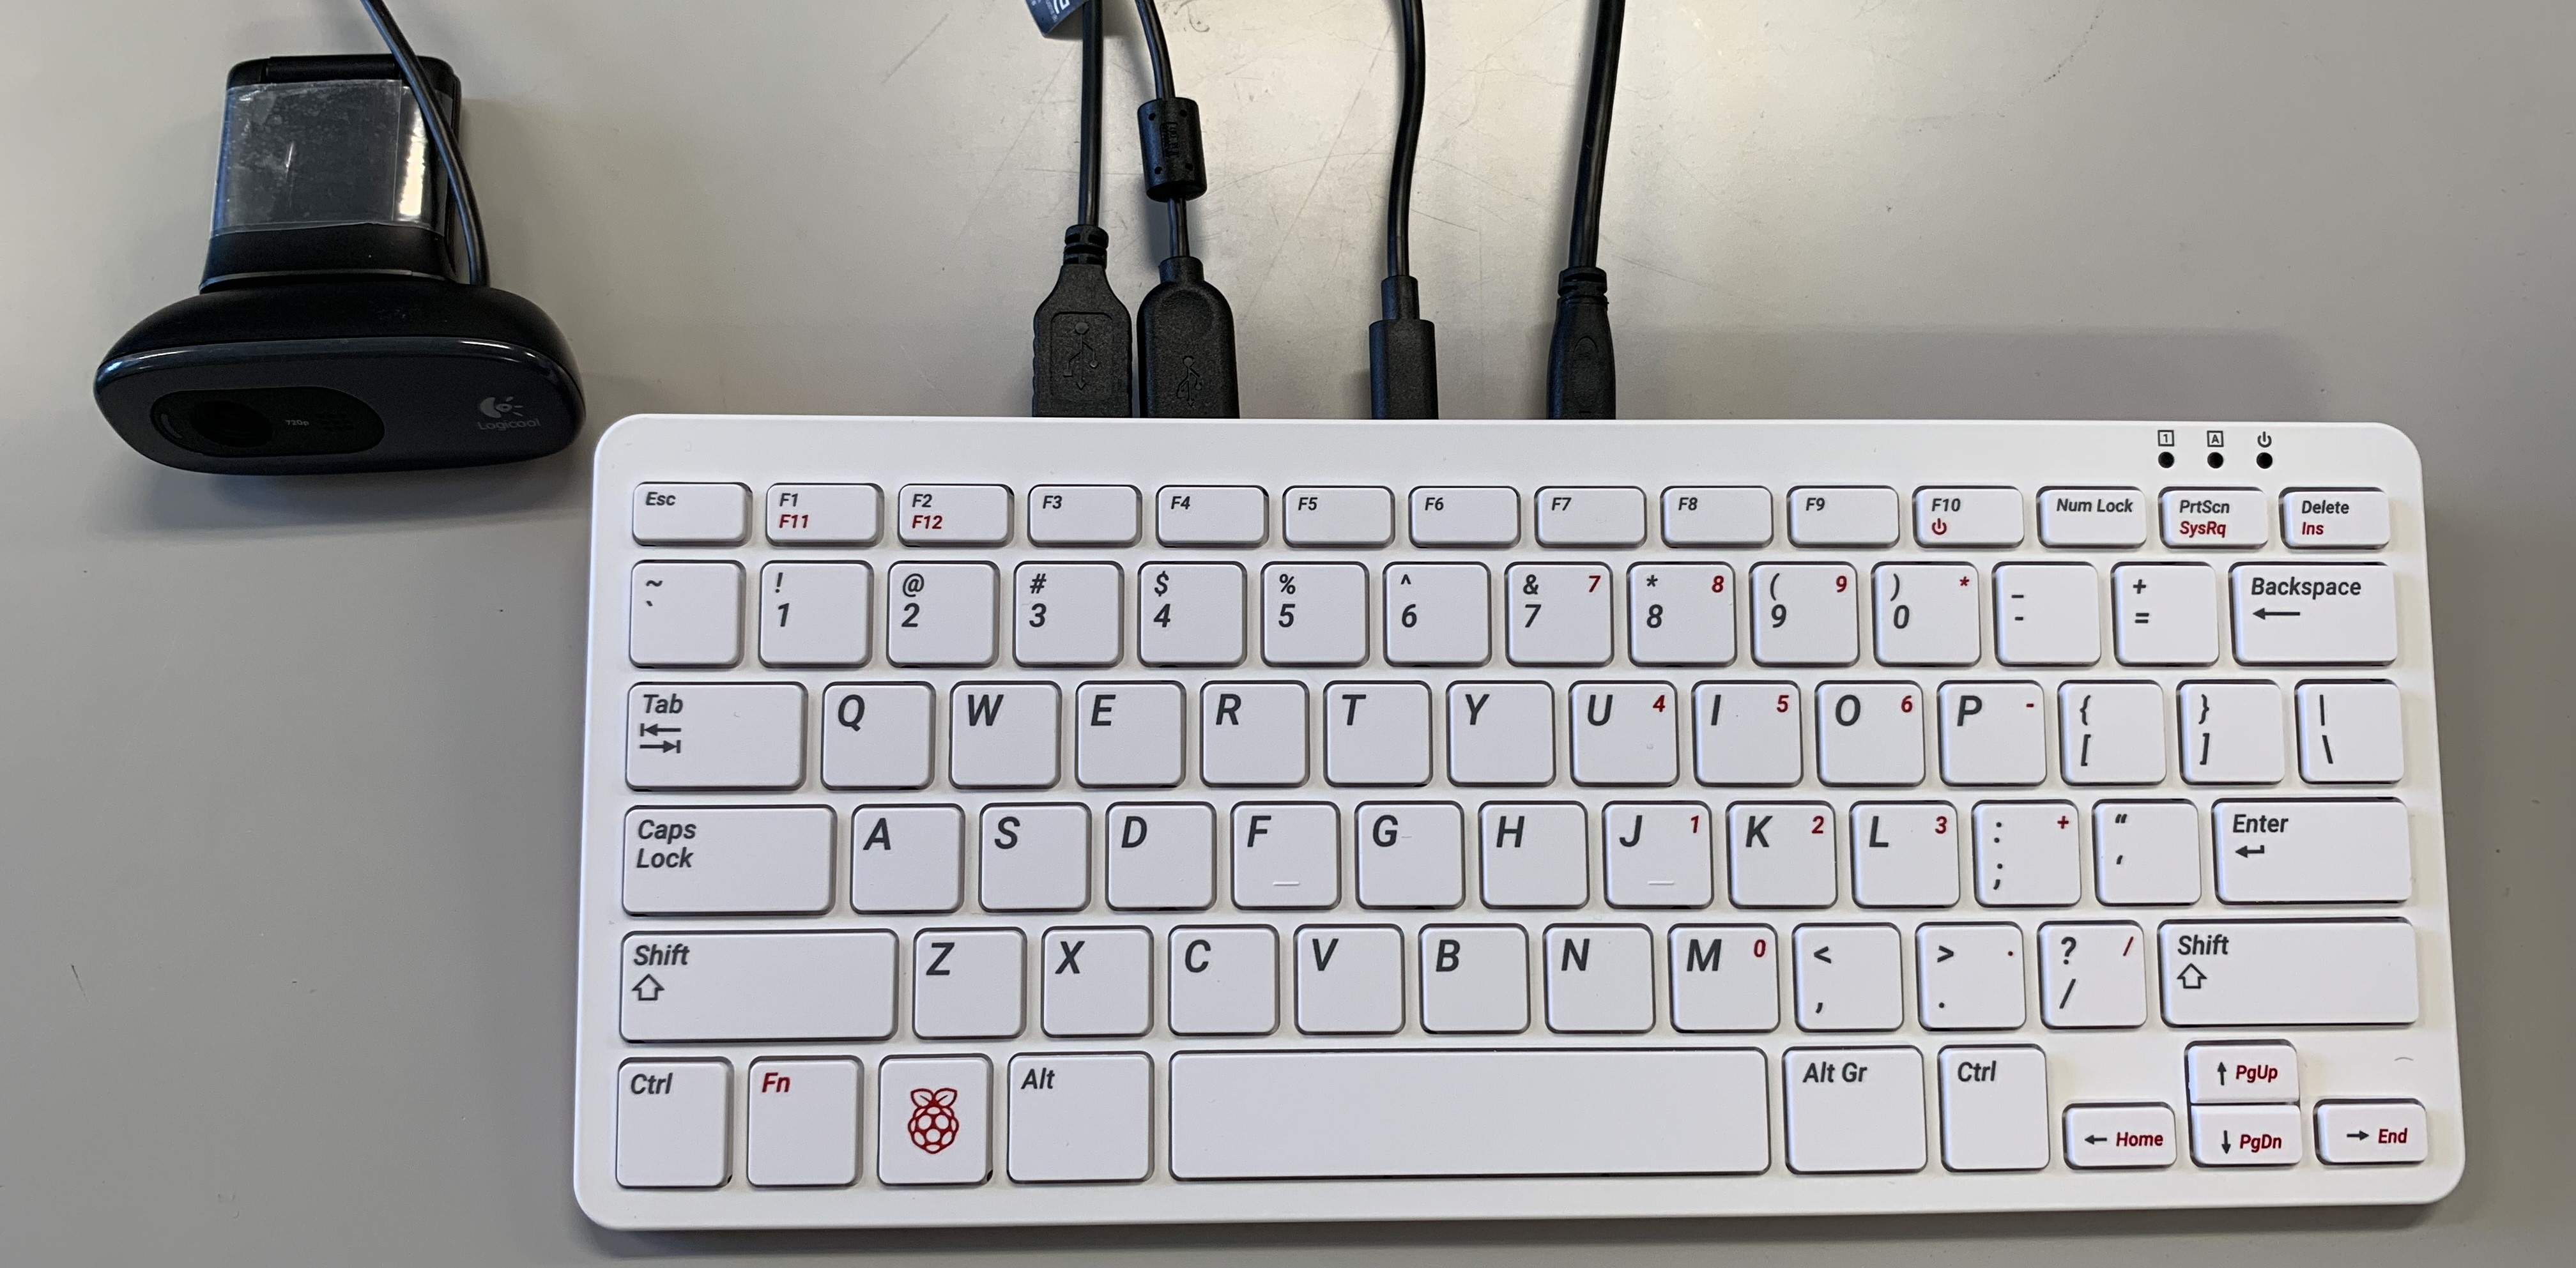
\includegraphics[width=0.8\textwidth]{slide03_003.jpg}
    \vfill
    \large\textbf{教科書の36p-39pをよんで、ウェブカメラでHPの自己紹介用に自分の顔写真をさつえいしよう}
    \vfill
    \large\textbf{わからないことは、放っておかず、すぐに TA に聞きましょう}
\end{frame}

\begin{frame}[fragile]
	\frametitle{例題1-16 カメラで写真をさつえいしよう P.36-39~~~\raisebox{-3mm}{
\includegraphics[width=0.1\textwidth]{raspberry}}}
    \large\textbf{ウェブカメラで撮影する前に}
    \begin{itemize}
      \item 人は誰でも私生活上の容姿を無断でさつえいされたり、さつえいされた写真や映像を勝手に公表されたりするのは不快であり、嫌悪感や恐怖を覚えるものです。
      \item 人は誰でも私生活上の情報を無断で公表されない権利を持っています。
      \item このような、勝手にさつえいされないように保護を受けることのできる権利を肖像権と言います。
    \end{itemize}
    \vfill
    \large\textbf{他人をむやみにとってはいけません}
    \vfill
    \large\textbf{HPの自己紹介用に自分の顔写真を撮影しよう}
\end{frame}

\begin{frame}[fragile]
	\frametitle{例題1-16 カメラで写真をさつえいしよう P.36-39~~~\raisebox{-3mm}{
\includegraphics[width=0.1\textwidth]{raspberry}}}
    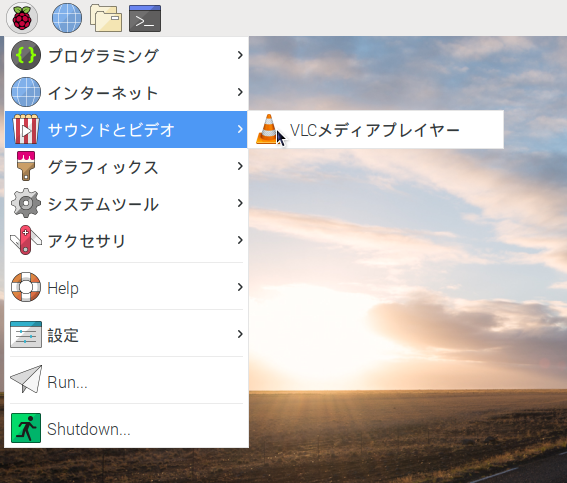
\includegraphics[width=0.47\textwidth]{textbook-img113.png}
    \hfill
    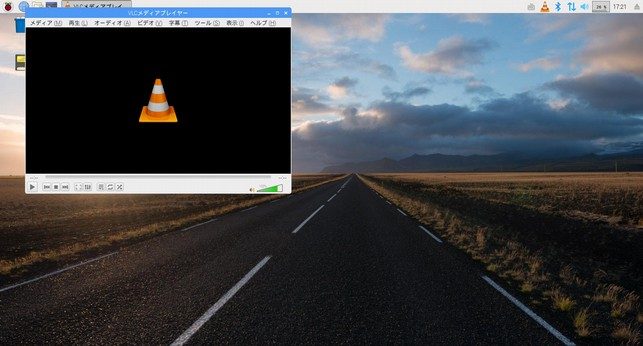
\includegraphics[width=0.47\textwidth]{textbook-img114.jpg}
    \vfill
    \large\textbf{写真のさつえいのやり方(1)}
    \begin{itemize}
      \item 「VLCメディアプレーヤー」を起動しよう
    \end{itemize}
\end{frame}

\begin{frame}[fragile]
	\frametitle{例題1-16 カメラで写真をさつえいしよう P.36-39~~~\raisebox{-3mm}{
\includegraphics[width=0.1\textwidth]{raspberry}}}
    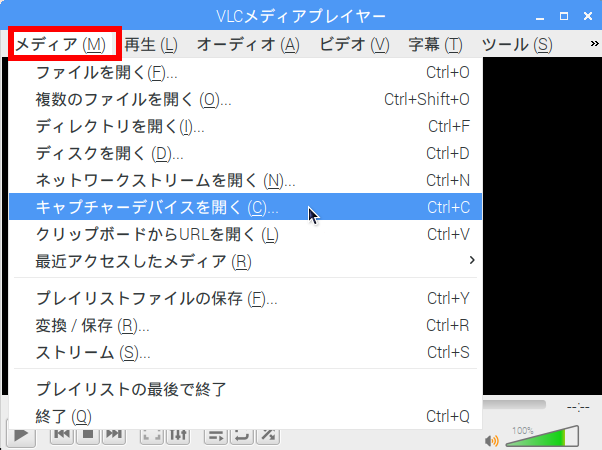
\includegraphics[width=0.37\textwidth]{textbook-img116.png}
    \hfill
    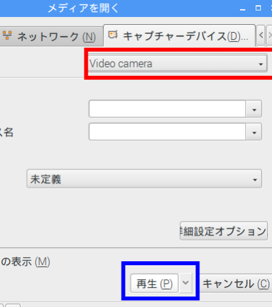
\includegraphics[width=0.3\textwidth]{slide03_004.png}
    \hfill
    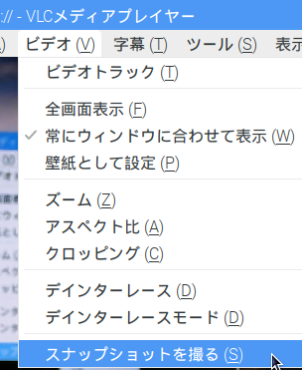
\includegraphics[width=0.3\textwidth]{slide03_005.png}
    \vfill
    \large\textbf{写真のさつえいのやり方(2)}
    \begin{itemize}
      \item カメラを起動しよう
      \item スナップショットをとろう
    \end{itemize}
\end{frame}

\begin{frame}[fragile]
	\frametitle{例題1-17 画像に絵をかこう P.40-43~~~\raisebox{-3mm}{
\includegraphics[width=0.1\textwidth]{raspberry}}}
  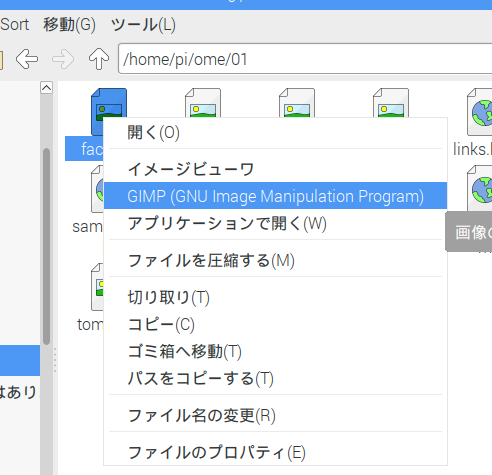
\includegraphics[width=0.35\textwidth]{textbook-img124.png}
  \hfill
  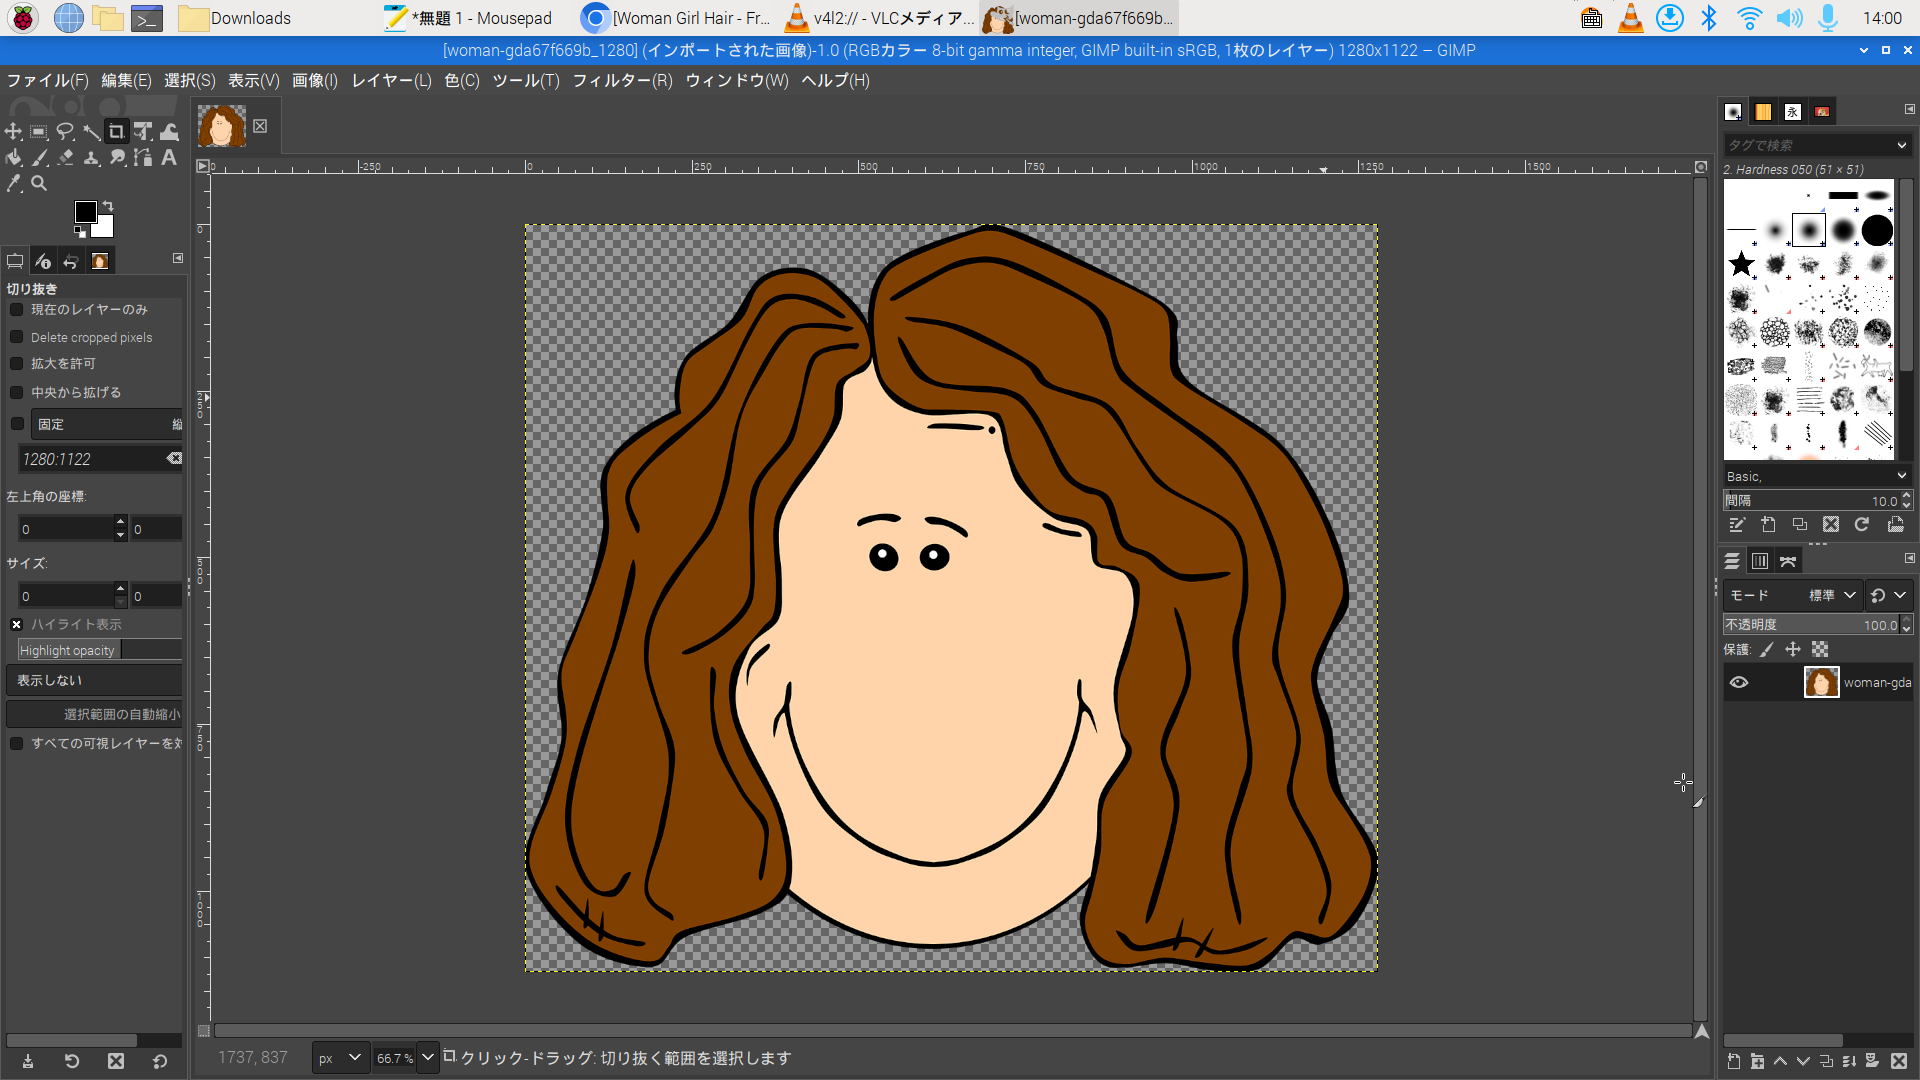
\includegraphics[width=0.62\textwidth]{textbook-img125.png}
  \vfill
  \large\textbf{教科書の40p-43pをよんで、画像に絵をかこう}
  \begin{itemize}
    \item 「GIMP」ソフトを立ち上げて、色付きの筆で自分の顔写真に絵をかこう
  \end{itemize}

\end{frame}

\begin{frame}[fragile]
	\frametitle{例題1-17 画像に絵をかこう P.40-43~~~\raisebox{-3mm}{
\includegraphics[width=0.1\textwidth]{raspberry}}}
          \large\textbf{教科書を読んで、問題にチャレンジしよう}
          \begin{itemize}
            \item 問題1-16
          \end{itemize}
          \vfill
          \large\textbf{わからないことは、放っておかず、すぐに TA に聞きましょう}
\end{frame}

\begin{frame}[fragile]
	\frametitle{\raisebox{-3mm}{
\includegraphics[width=0.1\textwidth]{raspberry}}休憩~~~\raisebox{-3mm}{
\includegraphics[width=0.1\textwidth]{raspberry}}}
	\huge
      \begin{itemize}
           \item 水分補給をしましょう
           \item 遠くのものを見て目を休めましょう
     \end{itemize}
\end{frame}

\end{document}
